\documentclass[conference]{IEEEtran}
\IEEEoverridecommandlockouts
\usepackage{cite}
\usepackage{amsmath,amssymb,amsfonts}
\usepackage{algorithmic}
\usepackage{graphicx}
\graphicspath{{figures/}}
\usepackage{textcomp}
\usepackage{xcolor}
\usepackage{booktabs}
\usepackage{multirow}
\def\BibTeX{{\rm B\kern-.05em{\sc i\kern-.025em b}\kern-.08em
    T\kern-.1667em\lower.7ex\hbox{E}\kern-.125emX}}
    
\begin{document}

\title{Performance Comparison of Docker and Kata-Firecracker for Web and Database Workloads}

\author{
\IEEEauthorblockN{Abhishek Mandal}
\IEEEauthorblockA{\textit{Department of Computer Science} \\
\textit{IIIT, Bangalore}\\
Bangalore, India}
\and
\IEEEauthorblockN{Sameer}
\IEEEauthorblockA{\textit{Department of Computer Science} \\
\textit{IIIT, Bangalore}\\
Bangalore, India }
}

\maketitle

\begin{abstract}
Virtual Machines (VMs) and containers are used extensively in cloud computing. While traditional containers like Docker offer excellent performance and low overhead, they raise security concerns due to shared host kernels. Lightweight hypervisors like Kata Containers utilizing Firecracker have emerged to strike a balance between strong isolation and high performance. This paper investigates the performance characteristics of Docker containers versus Kata-Firecracker by measuring startup time, memory footprint, CPU utilization, throughput, and latency on an Nginx web server and a MySQL database. We analyze the benchmarking results across 50 independent runs, discuss the implications of the trade-offs between isolation and speed, and identify the causal links between hardware virtualization traps (VM Exits) and throughput degradation.
\end{abstract}

\begin{IEEEkeywords}
Lightweight Hypervisor, Container, Virtualization, Firecracker, Docker, Performance Evaluation, Nginx, MySQL
\end{IEEEkeywords}

\section{Introduction}
Containers have been introduced to overcome the heavy overhead of traditional VMs, allowing hardware resources to be split efficiently to enhance utilization. However, containers expose a larger attack surface compared to VMs as they share the same host kernel. To address this, organizations have developed lightweight hypervisors to strike a balance between traditional VMs and containers. 

This study focuses on Amazon's Firecracker, a lightweight hypervisor tailored for serverless applications, and Docker, the standard containerization platform. We look at their performance across a high-level application aspect covering an Nginx web server and a MySQL database management system. 

\section{Methodology}
To evaluate the application performance, we benchmarked the Nginx web server and MySQL database in both Docker and Kata-Firecracker environments. 

\subsection{Execution Environment and Tooling}
The web server benchmarks were automated via a custom Python testing harness using \texttt{hey} which is a high-performance HTTP load generator written in Go, to flood the target containers with traffic. Each runtime environment was subjected to 50,000 HTTP requests at a concurrency level of 20, repeated across 50 independent runs to ensure statistical significance. Furthermore, strict CPU pinning and core allocation were enforced to eliminate host-level CPU contention. The Nginx containers (both Docker and Kata) were pinned to CPUs 2, 3, 6, and 7 with a strict memory limit of 1024 MB. To ensure host-level isolation, the hey load generator was restricted to CPUs 0, 1, 4, and 5.

For the database evaluation, we utilized \texttt{sysbench} 1.0.20 to run an \texttt{oltp\_read\_write} workload consisting of $\sim$70\% SELECT, $\sim$20\% INSERT, and $\sim$10\% UPDATE/DELETE queries. The database was populated with 4 tables of 100,000 rows each (400,000 total), and the test was executed with 4 threads for 60 seconds per run, preceded by a 30-second warmup, across 5 independent runs. To isolate storage I/O from virtualization overhead, Docker was tested under two configurations: standard host filesystem (overlay2 with a named volume and \texttt{O\_DIRECT} flushing) and RAM-backed storage (\texttt{tmpfs}). Kata-Firecracker used the devmapper snapshotter with a virtio-mmio block device. All configurations were allocated identical resources: 4 CPUs pinned to cores 0--3, with 4096 MiB of RAM.

\subsection{Telemetry and Metric Collection}
Standard host-based monitoring tools (\texttt{cgroups}) suffer from a visibility gap when observing microVMs, as the host kernel is blind to workloads executing inside the KVM boundary. To ensure accurate resource profiling, our testing harness utilized a multi-tiered sampling approach:

\begin{itemize}
    \item \textbf{Resource Utilization Tracking:} For standard Docker containers, we utilized the native Docker API to poll cgroup metrics. For Kata-Firecracker, we directly monitored the localized \texttt{firecracker} process ID (PID) via the host OS to accurately capture the aggregate CPU and memory footprint of the Virtual Machine Monitor (VMM).
    
    \item \textbf{Hardware Virtualization Traps:} To correlate performance degradation with hypervisor isolation, we utilized Linux \texttt{perf} attached directly to the container worker PIDs and the \texttt{firecracker} VMM. This allowed us to explicitly capture hardware-level context switches (\texttt{cs}) and KVM transitions (\texttt{kvm exits and kvm enters}).

    \item \textbf{Hypervisor Diagnostics:} To further categorize the root cause of the VM Exits, we sampled global KVM counters via \texttt{/sys/kernel/debug/kvm} before and after each run.
    
\end{itemize}

\section{Evaluation and Results: Nginx}

To ensure statistical rigor, the Nginx benchmarks were executed 50 times. The results discussed below represent the averages and distributions across these 50 independent runs, with strict CPU core pinning to ensure an isolated testing environment.

\subsection{Startup Time and Resource Footprint}
The virtualization tax of a microVM manifests primarily in its static resource footprint. Table \ref{tab:nginx_resources} highlights the boot time, CPU (percentage representing core saturation), and memory utilization for both environments. 

\begin{table}[htbp]
\caption{Nginx: Boot Time and Resource Utilization (50-Run Average)}
\begin{center}
\begin{tabular}{lccc}
\toprule
\textbf{Environment} & \textbf{Boot Time (ms)} & \textbf{CPU (\%)} & \textbf{Memory (MiB)} \\
\midrule
Docker & 519.74 & 178.79 & 6.03 \\
Kata-Firecracker & 520.72 & 67.73 & 187.34 \\
\bottomrule
\end{tabular}
\label{tab:nginx_resources}
\end{center}
\end{table}

Both runtimes achieve incredibly fast, nearly identical startup times of $\sim$520ms. However, the resource utilization characteristics diverge significantly. As shown in Fig. \ref{fig:nginx_memory}, Kata-Firecracker requires $\sim$187 MiB of memory to back the guest kernel, compared to Docker's minimal 6 MiB footprint.

\begin{figure}[htbp]
\centerline{\includegraphics[width=0.45\textwidth]{nginx_memory_box.png}} 
\caption{Memory footprint comparison between Docker and Kata-Firecracker across 50 runs.}
\label{fig:nginx_memory}
\end{figure}

\begin{figure}[htbp]
\centerline{\includegraphics[width=0.45\textwidth]{nginx_cpu_box.png}}
\caption{CPU utilization comparison demonstrating isolation bounds.}
\label{fig:nginx_cpu}
\end{figure}

\subsection{Throughput and Latency}
Table \ref{tab:nginx_throughput} summarizes the network performance and request latency.

\begin{table}[htbp]
\caption{Nginx: Throughput and Latency (50-Run Average)}
\begin{center}
\begin{tabular}{lccccc}
\toprule
\multirow{2}{*}{\textbf{Environment}} & \textbf{Throughput} & \multicolumn{4}{c}{\textbf{Latency (ms)}} \\
\cmidrule(lr){3-6}
& \textbf{(req/sec)} & \textbf{Avg} & \textbf{p50} & \textbf{p95} & \textbf{p99} \\
\midrule
Docker & 31,243.92 & 0.61 & 0.51 & 1.49 & 2.41 \\
Kata-Firecracker & 28,897.09 & 0.69 & 0.59 & 1.40 & 2.25 \\
\bottomrule
\end{tabular}
\label{tab:nginx_throughput}
\end{center}
\end{table}

As depicted in Fig. \ref{fig:nginx_throughput}, Docker achieves higher throughput, maintaining a 7.5\% advantage over Kata-Firecracker. 

\begin{figure}[htbp]
\centerline{\includegraphics[width=0.45\textwidth]{nginx_throughput_box.png}}
\caption{Nginx Web Server Throughput comparison across 50 runs.}
\label{fig:nginx_throughput}
\end{figure}

\begin{figure}[htbp]
\centerline{\includegraphics[width=0.45\textwidth]{nginx_latency_percentiles.png}}
\caption{Latency Percentiles (p50, p90, p95, p99).}
\label{fig:nginx_latency}
\end{figure}

\subsection{The Virtualization Tax: Correlating VM Exits to Performance Drop}
To understand the 7.5\% throughput degradation in Kata-Firecracker, we must analyze the interaction between the guest OS and the host OS. Fig. \ref{fig:nginx_context_switches} demonstrates a stark divide in host-level context switches. Docker operates natively on the host kernel, resulting in minimal context switching. Kata-Firecracker, however, induces massive context switching due to the hypervisor boundary.

\begin{figure}[htbp]
\centerline{\includegraphics[width=0.45\textwidth]{nginx_context_switches.png}}
\caption{Scatter plot of Context Switches vs. Throughput, highlighting the systemic overhead of hypervisor isolation.}
\label{fig:nginx_context_switches}
\end{figure}

This overhead is directly quantified by hardware virtualization traps, or VM Exits. Every time the Nginx worker process in the guest requires network I/O, the KVM intercepts the operation, forcing a VM Exit. Fig. \ref{fig:nginx_vm_exits} definitively correlates the frequency of these VM Exits to the reduction in throughput. The linear regression proves that as KVM traps increase, request processing capacity proportionally degrades, identifying VM Exits as the primary mechanism behind the virtualization tax.

\begin{figure}[htbp]
\centerline{\includegraphics[width=0.45\textwidth]{nginx_rps_vs_vm_exits.png}}
\caption{Scatter plot of Total VM Exits vs. Throughput for Kata-Firecracker, confirming the causal link between virtualization traps and performance degradation.}
\label{fig:nginx_vm_exits}
\end{figure}

To further dissect the exact architectural causes of these virtualization traps, we utilized \texttt{perf} hardware tracing during the HTTP load generation. As outlined in Table \ref{tab:kvm_exit_reasons} and visualized in Fig. \ref{fig:kvm_exit_reasons_perf}, the overhead is heavily dominated by the mechanics of network I/O emulation.

\begin{table}[htbp]
\caption{KVM Exit Reasons Breakdown (\texttt{perf} traced)}
\begin{center}
% \resizebox ensures the table never bleeds into the next column
\resizebox{\columnwidth}{!}{%
\begin{tabular}{lrlp{3.0cm}}
\toprule
\textbf{Reason} & \textbf{Avg Count} & \textbf{\%} & \textbf{Implication} \\
\midrule
\texttt{EPT\_MISCONFIG} & 30,174 & 37.0\% & MMIO/device emulation (\texttt{virtio-net}) \\
\texttt{MSR\_WRITE} & 26,742 & 32.8\% & Model-specific register writes \\
\texttt{HLT} & 17,768 & 21.8\% & vCPU idle/halted \\
\texttt{EXTERNAL\_INTERRUPT} & 4,362 & 5.3\% & Network packet interrupts \\
\texttt{PAUSE\_INSTRUCTION} & 1,599 & 2.0\% & Spinlock contention \\
\texttt{EPT\_VIOLATION} & 428 & 0.5\% & Page faults \\
\texttt{PREEMPTION\_TIMER} & 421 & 0.5\% & Timer preemption \\
\texttt{VMCALL} & 112 & 0.1\% & Hypercalls \\
\bottomrule
\end{tabular}%
}
\label{tab:kvm_exit_reasons}
\end{center}
\end{table}

\begin{figure}[htbp]
\centerline{\includegraphics[width=0.45\textwidth]{kvm_exit_reasons_perf.png}}
\caption{KVM Exit Reasons highlighting the dominance of MMIO device emulation and external interrupts.}
\label{fig:kvm_exit_reasons_perf}
\end{figure}

Our telemetry reveals that network-related virtualization traps account for approximately 42\% of all VM exits. The most frequent exit reason, \texttt{EPT\_MISCONFIG}, averaged 30,174 occurrences per run, comprising 37.0\% of the total exits. In the context of KVM and Firecracker, Extended Page Table (EPT) misconfigurations are triggered intentionally to handle Memory-Mapped I/O (MMIO). Every time the guest kernel interacts with the \texttt{virtio-net} ring buffer to transmit an HTTP response, it attempts to write to a memory address that KVM has configured to trap, forcing the hypervisor to step in and emulate the device. 

Additionally, \texttt{EXTERNAL\_INTERRUPT} exits averaged 4,362 per run (5.3\%), which represents the host hypervisor injecting virtual interrupts into the guest vCPU to signal the arrival of incoming HTTP requests from the load generator. This granular breakdown definitively proves that the hypervisor boundary intercepting the \texttt{virtio-net} device emulation is the primary mechanical cause of the throughput degradation, translating high-throughput network load directly into systemic CPU context-switching overhead.


\section{Evaluation and Results: MySQL}
Relational databases are highly stateful, I/O-intensive workloads that stress compute, memory, and storage paths simultaneously. We evaluated Transactions Per Second (TPS), Queries Per Second (QPS), and latency profiles across three configurations: Docker with standard disk storage, Docker with RAM-backed storage (tmpfs), and Kata-Firecracker with devmapper.

\subsection{MySQL Throughput}
Table~\ref{tab:mysql_results} summarizes the aggregate performance across 5 runs per environment. In the baseline comparison, Kata-Firecracker achieved 646.83 TPS while Docker on standard disk storage achieved 449.29 TPS, making Kata-Firecracker 44\% faster. This result is attributed to Docker's direct exposure to host disk I/O saturation, where disk utilization exceeded 95\% and await times reached 3 seconds, causing TPS to collapse below 100 in the worst intervals. Fig.~\ref{fig:mysql_diskio} illustrates this correlation during Docker's worst run, showing a sharp TPS collapse as disk utilization crosses 90\%. Kata-Firecracker's devmapper snapshotter, which uses block-level copy-on-write via a thin-provisioned pool, produced a smoother I/O pattern that avoided these stalls.

\begin{figure}[htbp]
\centerline{\includegraphics[width=0.45\textwidth]{mysql_disk_io_correlation.png}}
\caption{Docker (disk): inverse correlation between disk utilization and TPS during Run 2, showing I/O queue saturation causing throughput collapse.}
\label{fig:mysql_diskio}
\end{figure}

Docker on disk also exhibited a coefficient of variation (CV) of 19.3\% across runs, compared to Kata-Firecracker's 0.7\%. To eliminate disk I/O as a confounding variable and isolate the true virtualization overhead, Docker was re-benchmarked using RAM-backed storage (tmpfs). With disk contention removed, Docker on tmpfs achieved 843.51 TPS, which is 30.4\% faster than Kata-Firecracker, confirming the expected virtualization tax imposed by the microVM boundary. The latency profile follows a similar pattern: Kata-Firecracker and Docker tmpfs exhibit comparable P99 latencies of 10.61~ms and 9.76~ms respectively, while Docker on disk shows an inflated P99 of 41.69~ms due to I/O stalls.

\begin{table}[htbp]
\caption{MySQL \texttt{sysbench} OLTP Read/Write Results (5-Run Avg)}
\begin{center}
\begin{tabular}{lcccc}
\toprule
\textbf{Environment} & \textbf{TPS} & \textbf{Avg Lat} & \textbf{P99 Lat} & \textbf{CV} \\
 & & \textbf{(ms)} & \textbf{(ms)} & \\
\midrule
Docker (disk) & 449.29 & 9.36 & 41.69 & 19.3\% \\
Kata-Firecracker & 646.83 & 6.18 & 10.61 & 0.7\% \\
Docker (tmpfs) & 843.51 & 4.74 & 9.76 & 2.3\% \\
\bottomrule
\end{tabular}
\label{tab:mysql_results}
\end{center}
\end{table}

Fig.~\ref{fig:mysql_tps} and Fig.~\ref{fig:mysql_qps} visualize the throughput disparity across all three configurations. Docker on tmpfs operates at the highest throughput, while Kata-Firecracker maintains a consistent but lower baseline due to the microVM boundary.

\begin{figure}[htbp]
\centerline{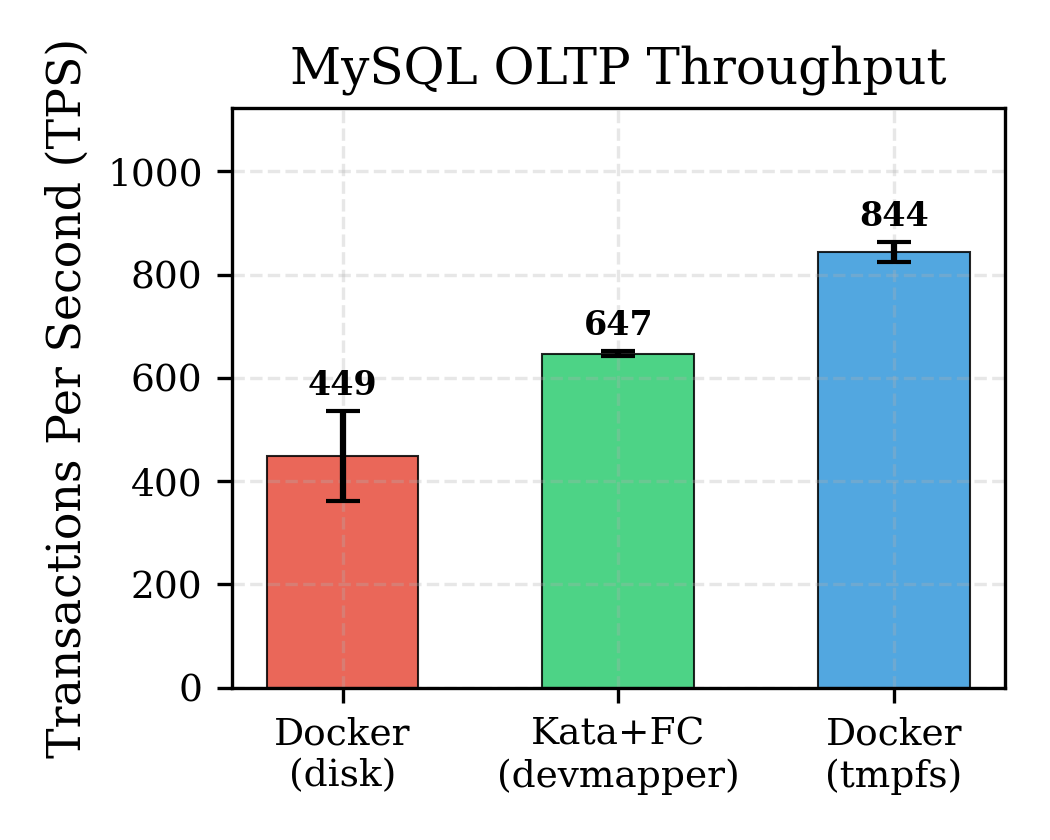
\includegraphics[width=0.45\textwidth]{mysql_tps_comparison.png}}
\caption{MySQL Transactions Per Second (TPS) comparison.}
\label{fig:mysql_tps}
\end{figure}

\begin{figure}[htbp]
\centerline{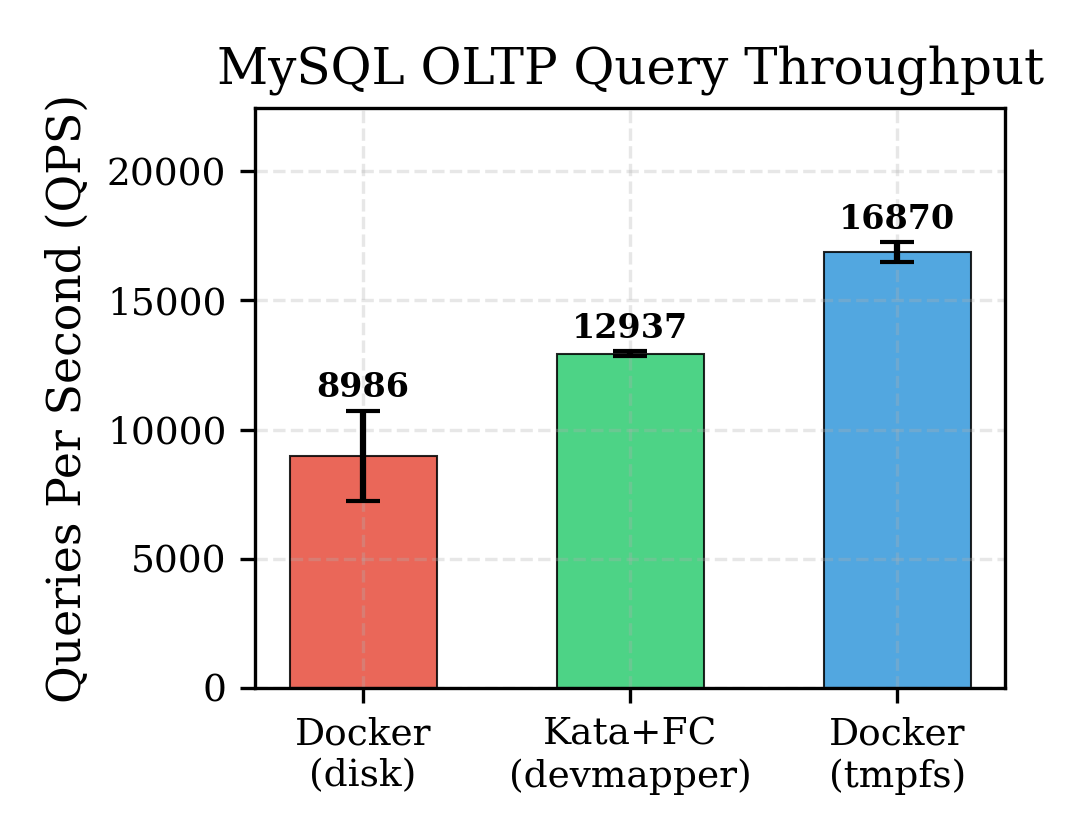
\includegraphics[width=0.45\textwidth]{mysql_qps_comparison.png}}
\caption{MySQL Queries Per Second (QPS) comparison.}
\label{fig:mysql_qps}
\end{figure}

\subsection{MySQL Latency and Stability}
Fig.~\ref{fig:mysql_latency} presents the latency profile on a logarithmic scale. While minimum and average latencies are comparable across Docker tmpfs and Kata-Firecracker, Docker on disk exhibits dramatically worse P99 (41.69~ms) and maximum latency (184.40~ms) due to I/O stalls. To verify throughput stability under sustained load, 10-second interval measurements were captured over the 60-second test duration. As shown in Fig.~\ref{fig:mysql_tps_time}, Kata-Firecracker delivers remarkably flat throughput ($\sim$640--665 TPS across all intervals), while Docker on disk shows severe oscillations between 296 and 668 TPS as disk I/O saturates. Docker on tmpfs maintains high throughput throughout with a gentle upward trend as the InnoDB buffer pool warms.

\begin{figure}[htbp]
\centerline{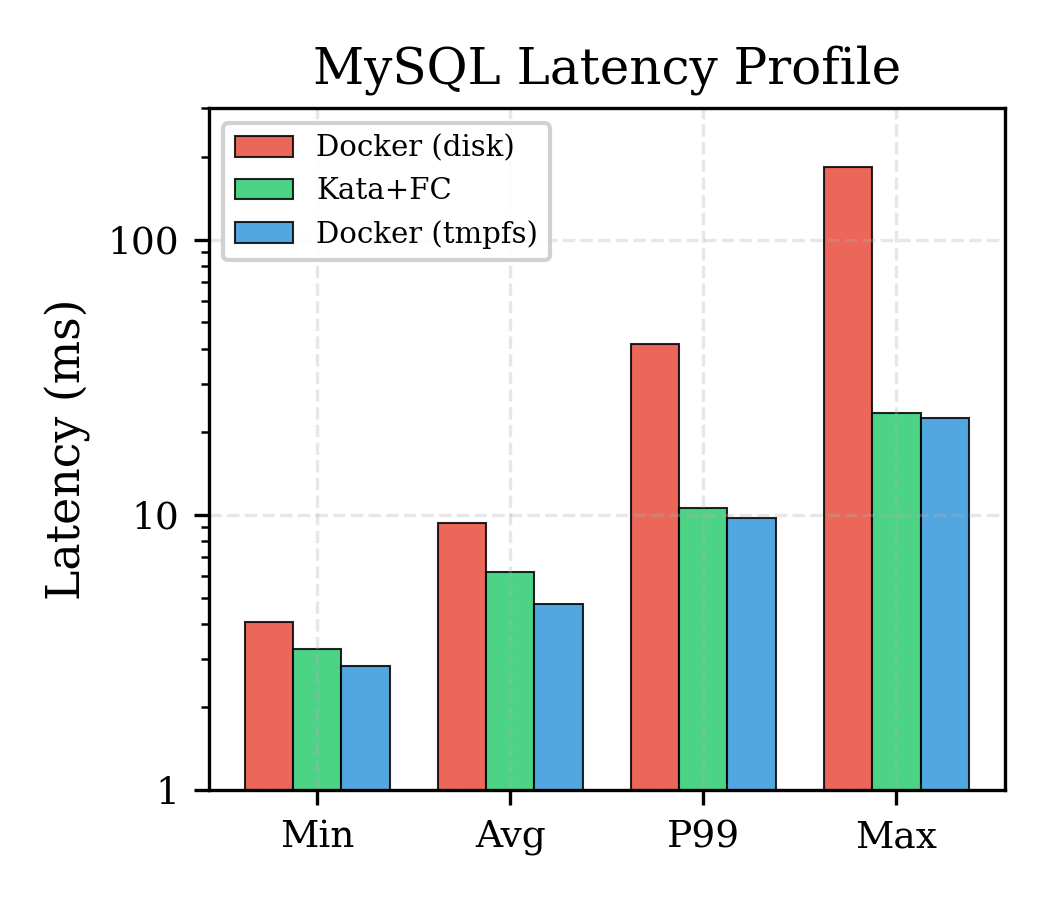
\includegraphics[width=0.45\textwidth]{mysql_latency_profile.png}}
\caption{MySQL latency profile comparison (log scale): Min, Avg, P99, and Max.}
\label{fig:mysql_latency}
\end{figure}

\begin{figure}[htbp]
\centerline{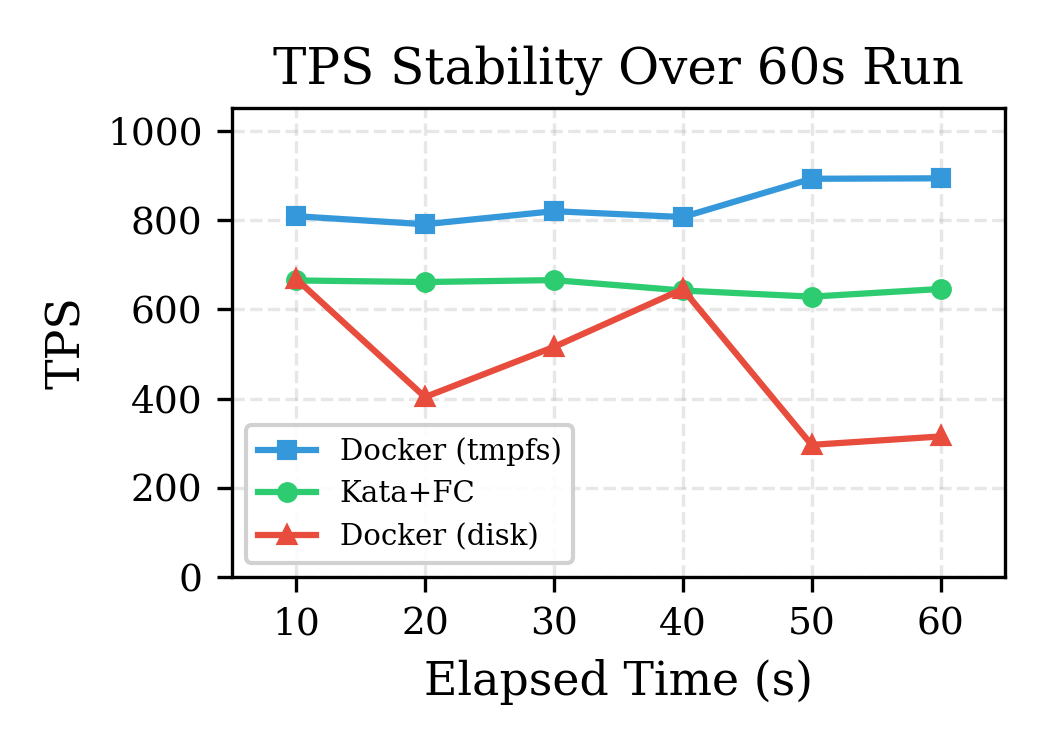
\includegraphics[width=0.45\textwidth]{mysql_tps_over_time.png}}
\caption{TPS stability over a 60-second run, showing Kata-Firecracker's flat profile versus Docker on disk's I/O-induced oscillations.}
\label{fig:mysql_tps_time}
\end{figure}

\subsection{VM-Exit Root Cause Analysis}
To quantify the virtualization tax in Kata-Firecracker, we captured hardware-level KVM exit counters via \texttt{/sys/kernel/debug/kvm/} and used \texttt{perf kvm stat} to classify exit reasons. On average, each 60-second run generated $\sim$3.4 million VM exits, yielding $\sim$87 exits per transaction. Fig.~\ref{fig:mysql_vmexit} shows the breakdown. MSR (Model-Specific Register) accesses dominate by count (44\%, avg 5.17~$\mu$s each), triggered by guest timer and performance counter reads. However, HLT exits, though only 14\% by count, consume 69\% of total exit handling time at 110.55~$\mu$s average, as the hypervisor must context-switch the vCPU. NPF (Nested Page Fault) exits account for 15\% of samples and 11\% of time, reflecting memory virtualization overhead. Interrupt injection adds 22\% by count and 9\% by time.

\begin{figure}[htbp]
\centerline{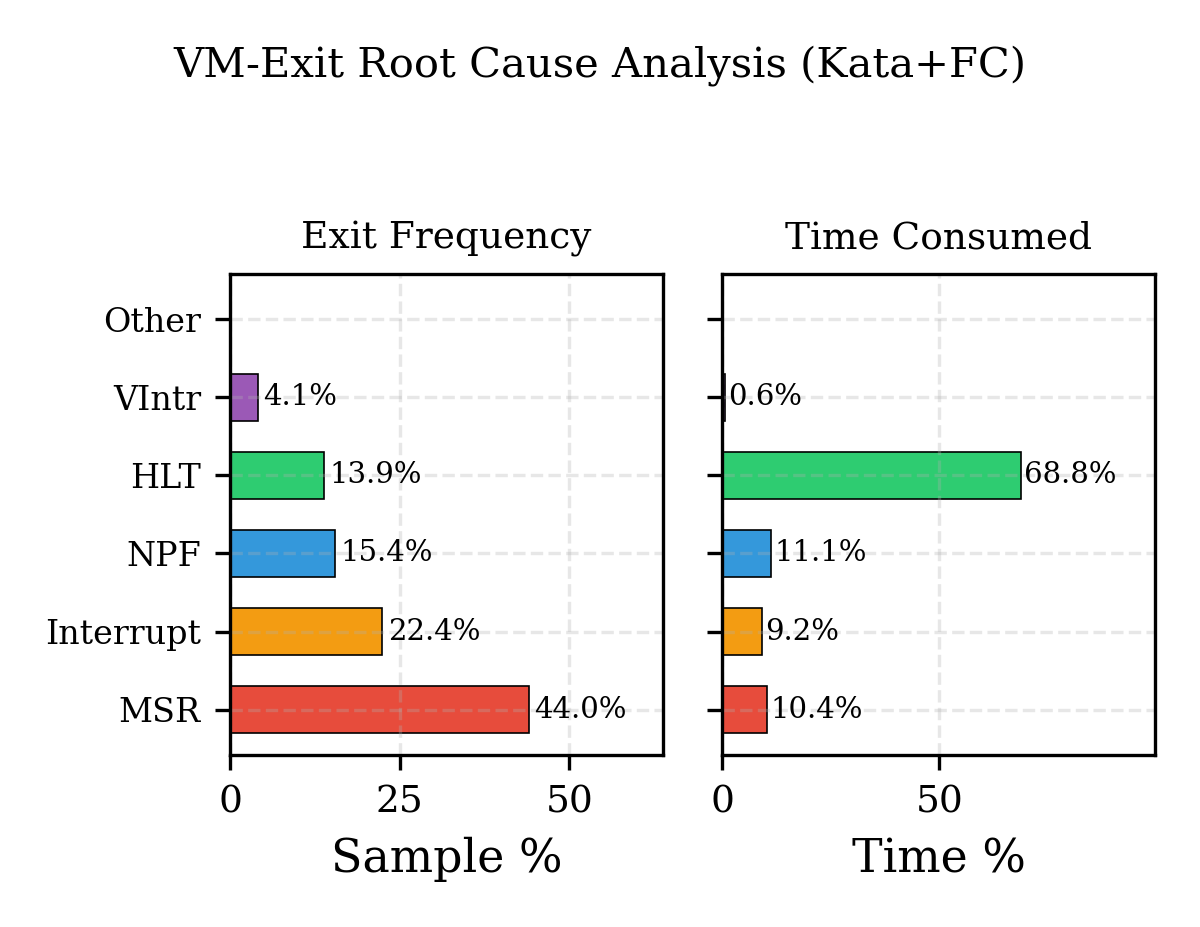
\includegraphics[width=0.45\textwidth]{mysql_vmexit_breakdown.png}}
\caption{VM-Exit root cause analysis for Kata-Firecracker: exit frequency (left) versus time consumed (right).}
\label{fig:mysql_vmexit}
\end{figure}

\subsection{Performance Variance Investigation}
While switching to tmpfs reduced Docker's CV from 19.3\% to 2.3\%, this remained $3{\times}$ higher than Kata-Firecracker's 0.7\%. Fig.~\ref{fig:mysql_var} visualizes the TPS distribution across all three environments, highlighting the residual variance gap between Docker tmpfs and Kata-Firecracker.

\begin{figure}[htbp]
\centerline{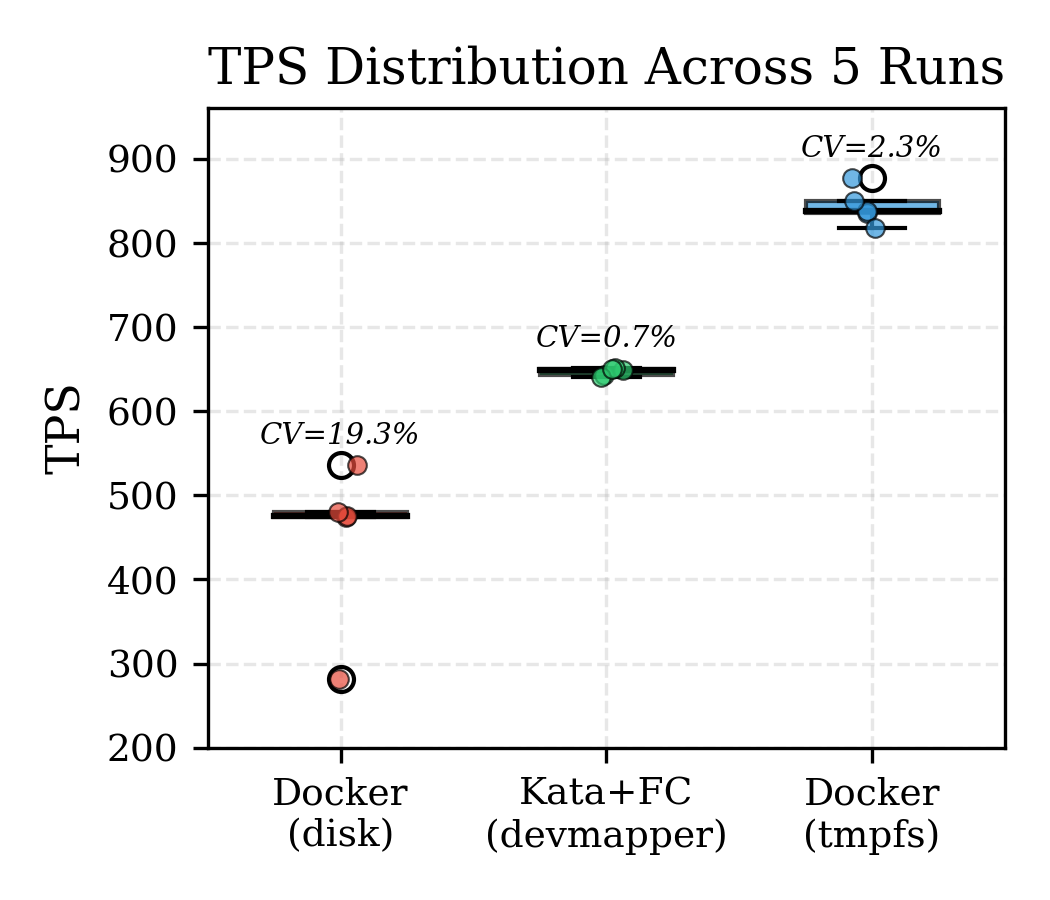
\includegraphics[width=0.45\textwidth]{mysql_tps_variability_box.png}}
\caption{TPS distribution across 5 runs showing variance characteristics.}
\label{fig:mysql_var}
\end{figure}

To identify the residual variance source, we designed a controlled isolation test with four phases sharing the same live MySQL container on tmpfs, eliminating warmup confounds. We tested two hypotheses: (H1)~Transparent Huge Page (THP) compaction and NUMA rebalancing cause multi-millisecond scheduling stalls, and (H2)~host daemon processes and IRQ handlers contend for the CPU cores pinned to the benchmark. Fig.~\ref{fig:mysql_iso} shows the results. Disabling THP (H1) reduced CV from 3.9\% to 1.1\%, identifying kernel memory compaction as the primary jitter source. CPU isolation via systemd cgroup slices and IRQ affinity (H2) further reduced CV to 0.5\%. The combined configuration (H3) achieved 0.4\% CV, converging with Kata-Firecracker's 0.7\%. This demonstrates that the microVM boundary in Kata-Firecracker implicitly provides the CPU and memory isolation that Docker requires explicit host-level tuning to achieve.

\begin{figure}[htbp]
\centerline{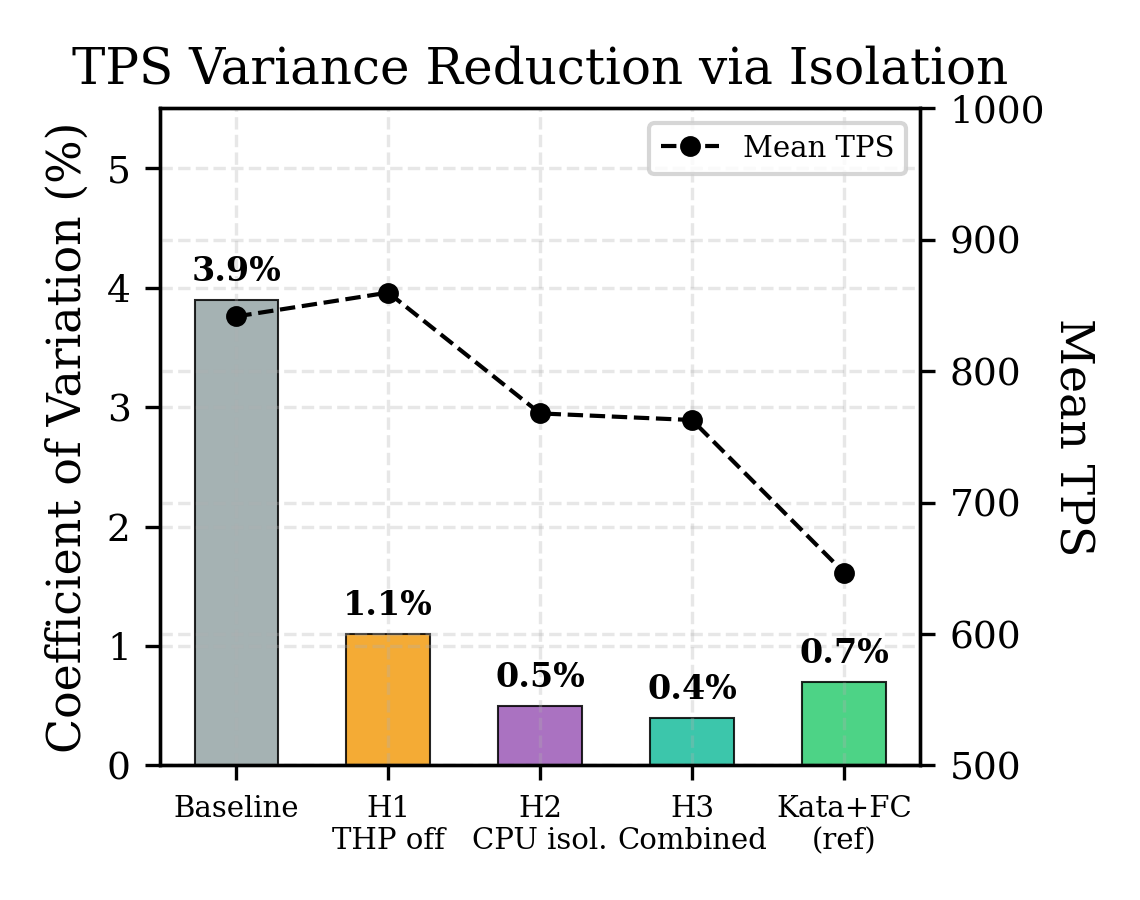
\includegraphics[width=0.45\textwidth]{mysql_isolation_cv.png}}
\caption{TPS variance reduction through incremental host isolation, converging with Kata-Firecracker's natural isolation.}
\label{fig:mysql_iso}
\end{figure}

\section{Discussion}
The benchmark results highlight a critical distinction in how lightweight hypervisors handle different types of computing workloads.

\textbf{Web Server Efficiency:} Docker handles stateless Nginx workloads with native efficiency, achieving over 31,000 requests per second. Kata-Firecracker, operating within a MicroVM boundary, introduces context-switching overhead resulting in a remarkably low $\sim$7.5\% reduction in HTTP throughput. Our analysis identified hardware virtualization traps (VM Exits) as the direct cause of this degradation. Every network I/O operation forces the CPU to trap out of the guest kernel, incurring a microsecond-level penalty that cumulatively reduces overall capacity. For lightweight web traffic, Firecracker's strong hardware isolation is well worth the minimal 7.5\% performance tax.

\textbf{Database Workloads and Isolation:} The MySQL results reveal a more nuanced narrative than a simple throughput comparison. When storage I/O is equalized via tmpfs, Docker outperforms Kata-Firecracker by 30.4\%, a direct consequence of the $\sim$3.4 million VM exits per run, dominated by HLT exits consuming 69\% of exit handling time. However, this throughput advantage comes at the cost of predictability. Docker on the host kernel is exposed to THP compaction stalls, host daemon CPU contention, and interrupt interference, factors that Kata-Firecracker's microVM boundary inherently isolates against. Our controlled isolation experiment demonstrated that manually replicating Kata-Firecracker's isolation properties on Docker (by disabling THP and restricting host processes to non-benchmark cores) reduces Docker's CV to match Kata-Firecracker's 0.7\%. This suggests that the ``overhead'' of a microVM is partially offset by the deterministic execution environment it provides, a property critical for latency-sensitive production database deployments.

\section{Conclusion}
This study evaluated the performance trade-offs between Docker and Kata-Firecracker across web server and database workloads. For HTTP workloads on Nginx, Kata-Firecracker trails Docker's throughput by only 7.5\% while providing hardware-level isolation and improved tail latency predictability. For database workloads, Docker achieves 30.4\% higher MySQL throughput when storage I/O is equalized, but exhibits $3{\times}$ higher performance variance. Our systematic variance investigation identified THP compaction, host daemon contention, and IRQ interference as the primary sources of Docker's jitter. By manually applying the isolation that Kata-Firecracker provides inherently through its microVM boundary, Docker's variance converges to match Kata-Firecracker's.

Beyond performance, Kata-Firecracker provides a fundamentally stronger security posture. Each container runs atop its own dedicated guest kernel inside a lightweight VM, meaning a kernel-level exploit within the container cannot compromise the host or neighboring workloads. Docker containers, by contrast, share the host kernel directly; any vulnerability in the shared kernel exposes all co-located containers to lateral attacks. Given that hundreds of Linux kernel CVEs are disclosed annually, this architectural difference is significant for multi-tenant deployments. The choice between Docker and Kata-Firecracker is therefore a trade-off between peak throughput and the combined benefits of security, isolation, and execution determinism. For latency-sensitive, multi-tenant production environments, particularly databases, Kata-Firecracker's moderate performance cost is justified by the inherent stability and strong isolation it provides without requiring manual host-level tuning.

\begin{thebibliography}{00}
\bibitem{b1} G. Li et al., ``Comparative Performance Study of Lightweight Hypervisors Used in Container Environment,'' in \textit{Proceedings of the 11th International Conference on Cloud Computing and Services Science (CLOSER 2021)}, pp. 215-223, 2021.
\bibitem{b3} A. Agache, M. Brooker, A. Florescu, A. Iordache, A. Liguori, R. Neugebauer, P. Piwonka, and D.-M. Popa, ``Firecracker: Lightweight Virtualization for Serverless Applications,'' in \textit{Proceedings of the 17th USENIX Symposium on Networked Systems Design and Implementation (NSDI '20)}, Santa Clara, CA, USA, Feb. 2020.
\end{thebibliography}

\end{document}
